
\noindent\begin{minipage}{\textwidth}
    \begin{table}[H]
        \centering
        \caption{Hiperparâmetros e Resultados do Melhor Modelo - vit\_v12\_BR\_opt\_aug}
        \vspace{0.2cm}
        \resizebox{\textwidth}{!}{%
            \begin{tabular}{ll | lrrr}
                \hline
                \multicolumn{2}{c|}{\textbf{Hiperparâmetros}} & \multicolumn{4}{c}{\textbf{Métricas por Classe}} \\ \hline
                \textbf{Parâmetro} & \textbf{Valor} & \textbf{Classe} & \textbf{Precisão} & \textbf{Recall} & \textbf{F1-Score} \\ \hline
    Agendador (Patience) & 8 & 31.2 & 0.3368 & 0.5766 & 0.4252 \\ 
Agendador de LR & ReduceLROnPlateau & 31.3 & 0.2698 & 0.1809 & 0.2166 \\ 
Architecture & vit\_b\_16 & 31.4 & 0.2672 & 0.1360 & 0.1802 \\ 
Batch Size & 32 & 32.3 & 0.2511 & 0.3069 & 0.2762 \\ 
Data Augmentation & False & 32.4 & 0.0500 & 0.0833 & 0.0625 \\ 
Decaimento de Peso (WD) & 0.0180 & 33.3 & 0.2577 & 0.1944 & 0.2216 \\ 
Dropout & 0.0067 & 41.4 & 0.0889 & 0.0851 & 0.0870 \\ 
Função de Perda & CrossEntropyLoss & 41.5 & 0.3684 & 0.3256 & 0.3457 \\ 
Hidden Units & 256 & 42.4 & 0.0753 & 0.1148 & 0.0909 \\ 
Label Smoothing & 0.0466 & 44.4 & 0.2000 & 0.0625 & 0.0952 \\ 
\cline{3-6} 
Otimizador & AdamW & \textbf{Média (Macro)} & 0.2380 & 0.2492 & 0.2126 \\ 
Taxa de Aprendizado (LR) & 1.33e-05 & \textbf{MCC} & \multicolumn{3}{c}{0.1737} \\ 
Unfreeze Layers & 2 &  & & &  \\ 
            \hline
            \end{tabular}%
        }
    \end{table}

    \begin{figure}[H]
        \centering
        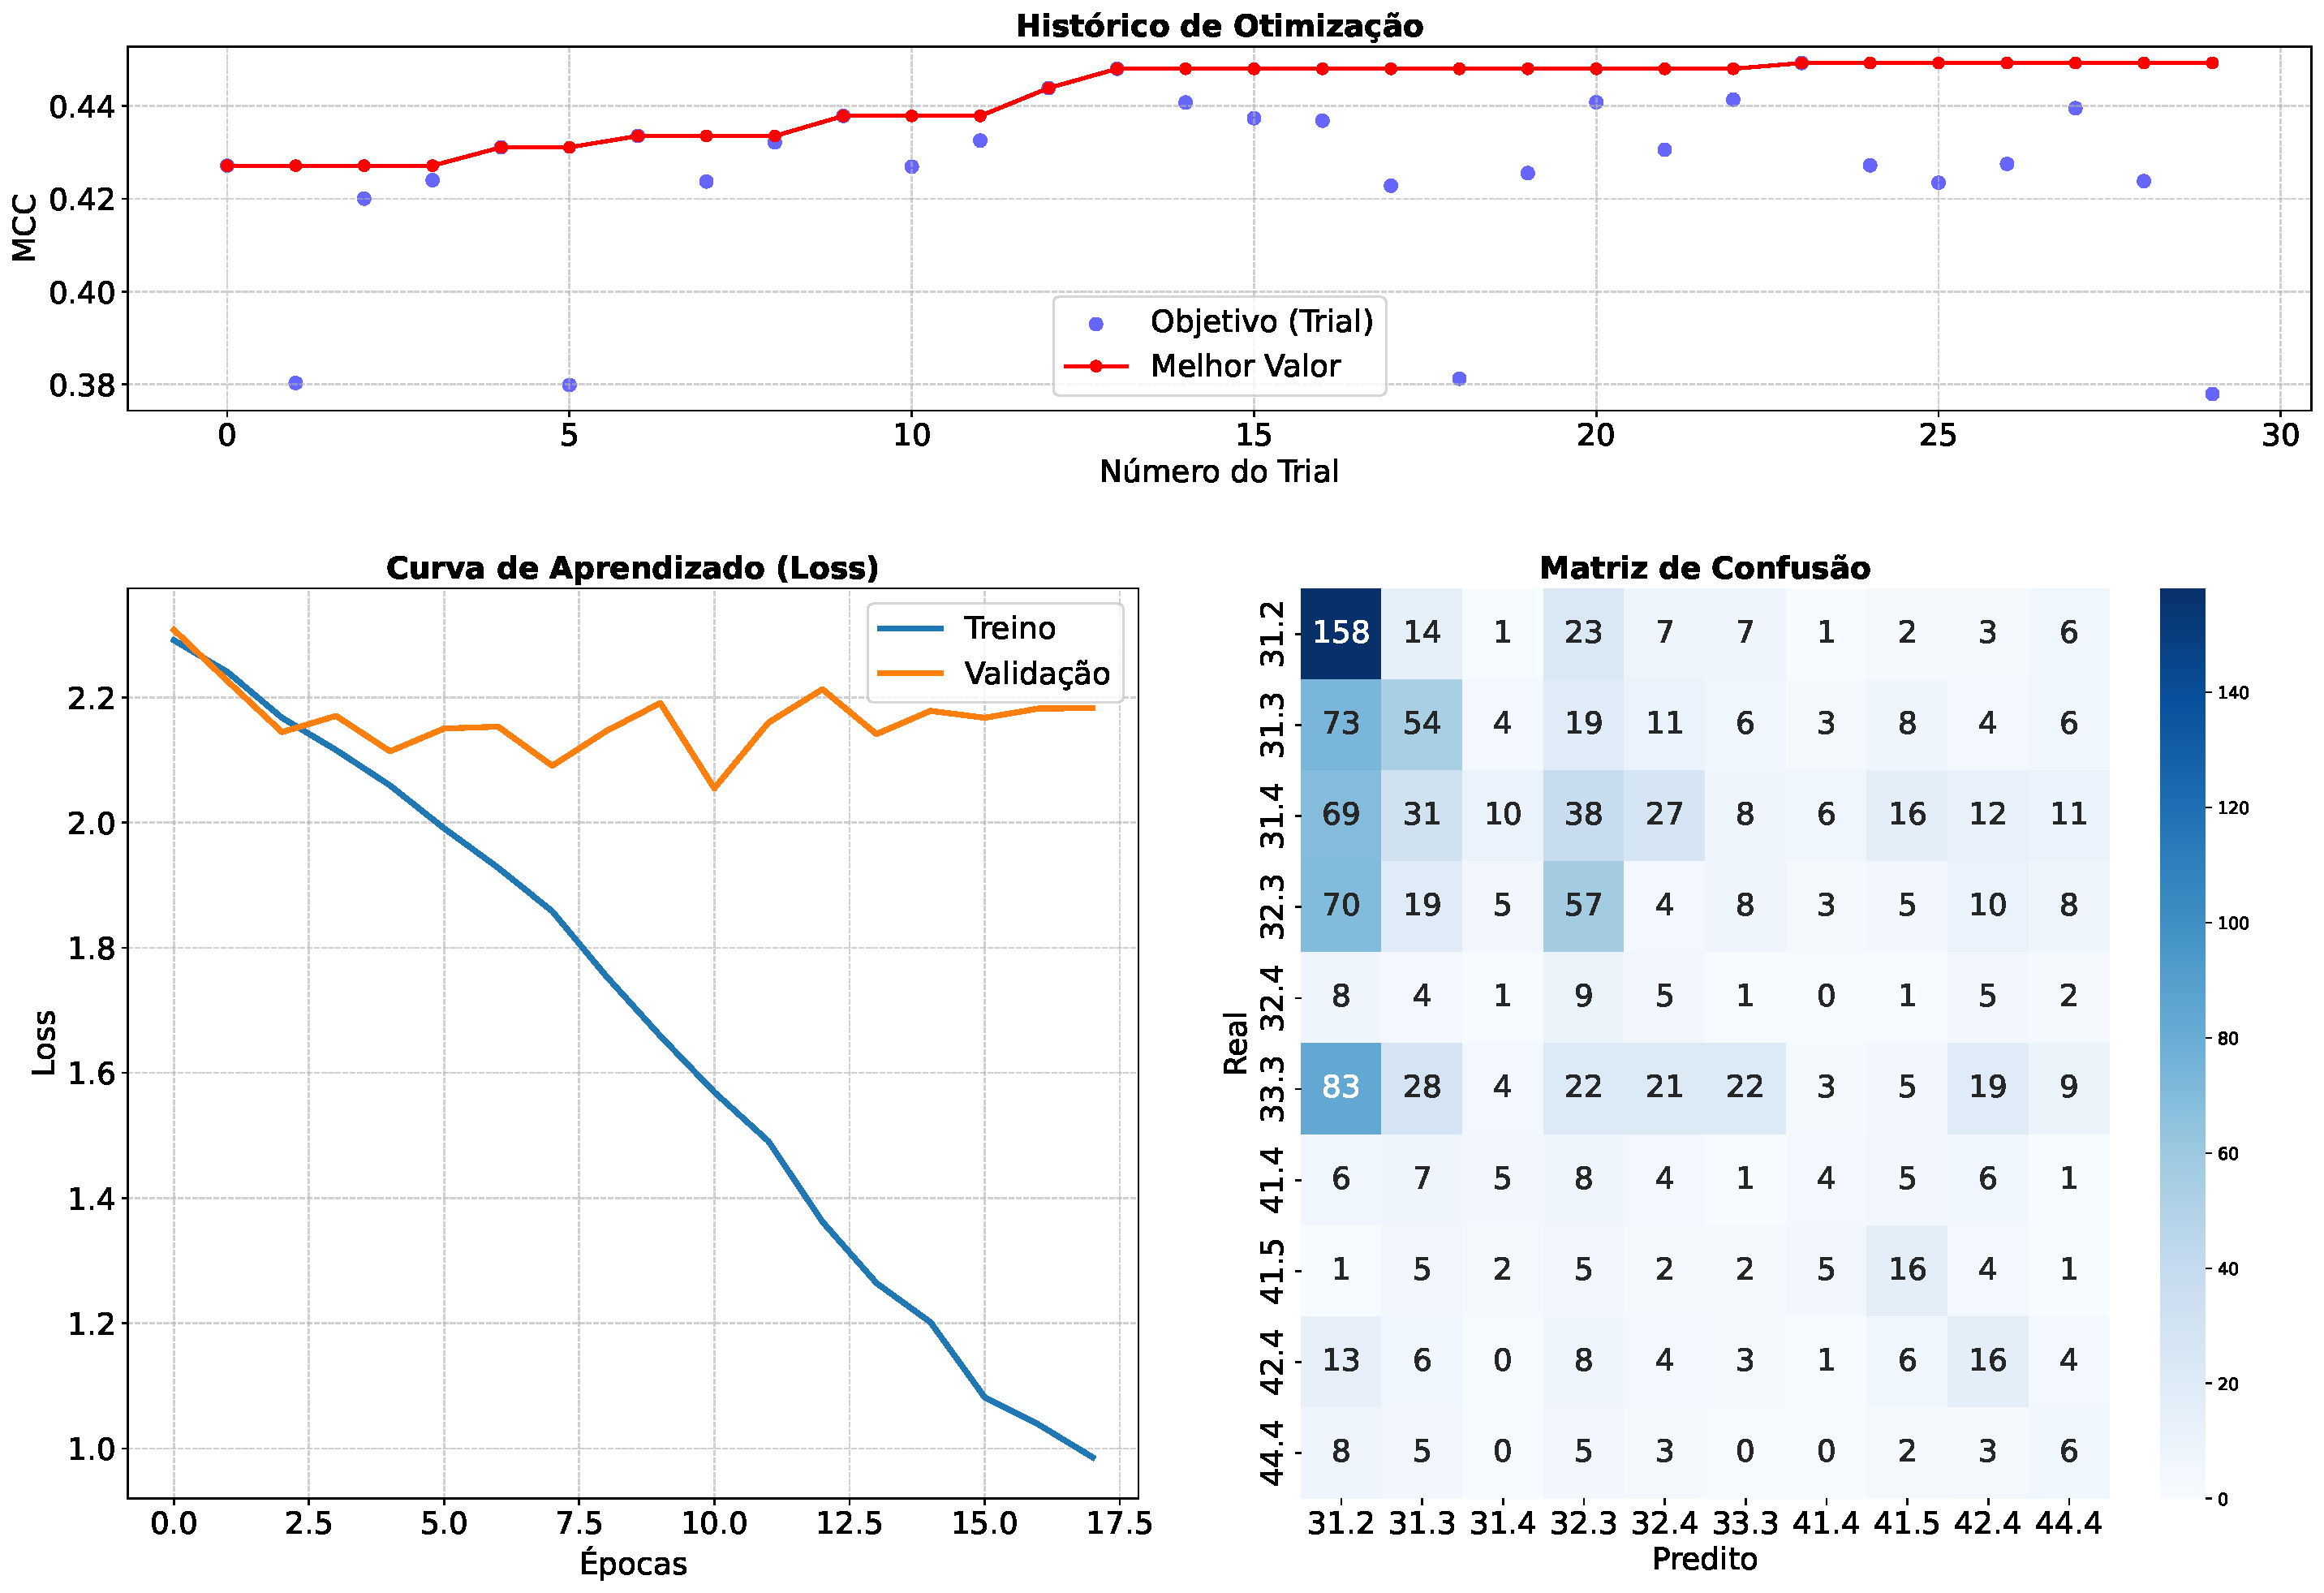
\includegraphics[width=0.85\textwidth]{tex/appendix/experiments/vit_v12_BR_opt_aug/dashboard_consolidado.pdf}
        \caption{Histórico de Otimização, Curvas de Aprendizado e Matriz de Confusão - vit\_v12\_BR\_opt\_aug}
    \end{figure}
\end{minipage}
\clearpage
